\documentclass[notes,color]{sepslide0}
\usepackage{graphicx}
\usepackage[overheads]{mysepslides}
\usepackage{tech,graphicx,url,tikz,scalalistings}

\title{Concurrent Datatypes} 
\author{Gavin Lowe}

\def\scalacolour{\color{violet}}

\begin{document}

\begin{slide}
  
  \Title


\end{slide}

%%%%%

\begin{slide}
\heading{Concurrent datatypes}

A \emph{concurrent datatype} is a datatype (e.g.~a queue, stack, set or
mapping) that can be safely accessed concurrently by multiple threads.
Operation invocations should appear to take place in a one-at-a-time order,
without interference. 

Threads that use the concurrent datatype can act much as they would with a
sequential datatype: the implementer of the threads does not need to think
much about concurrency.  

The implementer of the concurrent datatype \emph{does} have to think about
concurrency, and ensure different operation calls do not interfere with one
another.  But that concurrency is local, often inside a single object: local
reasoning is much easier than global reasoning.  And there's a lot of scope
for re-using concurrent datatypes.

Datatype-based concurrent programming encapsulates \emph{all} the concurrency
within a small number of concurrent datatypes.
\end{slide}

%%%%%

\begin{slide}
\heading{Example: a concurrent queue}

We will implement a concurrent queue.

What interface should a concurrent queue have?  A sequential queue would
typically have an interface like:

\begin{scala}
trait Queue[T]{
  /** Enqueue x. */
  def enqueue(x: T): Unit

  /** Dequeue a value.  
    * Pre: the queue is not empty. */
  def dequeue: T

  /** Is the queue empty? */
  def isEmpty: Boolean
}
\end{scala}
\end{slide}

%%%%% 

\begin{slide}
\heading{Example: a concurrent queue}

Client code is expected to check that the queue is non-empty before calling
|dequeue|:
\begin{scala}
  if(queue.isEmpty){ 
    ... // handle the empty queue
  } 
  else{ 
    val x = queue.dequeue; ... // do something with x
  }
\end{scala}

What happens if we use this approach  with a concurrent queue?
\end{slide} 

%%%%%


%% \begin{slide}
%% \heading{Example: a concurrent queue}

%% With the code on the previous slide, a thread~$A$ could call |queue.isEmpty|
%% and find that the queue is non-empty.  But before it performs the |dequeue|,
%% another thread could remove the last element from the queue.  Then when $A$
%% does perform the |dequeue|, the precondition is not satisfied.

%% This is sometimes called \emph{time-of-check to time-of-use} (TOCTTOU): there
%% is a gap between the check (that the queue is non-empty), and the operation
%% that depends upon that check (the dequeue), which means that the result of the
%% check may no longer be valid.
%% \end{slide}


%%%%%

\begin{slide}
\heading{Dealing with preconditions}

There are two main ways of dealing with operations that have a non-trivial
natural precondition.
%
\begin{itemize}
\item Return a special value to indicate that the natural precondition does
not hold.
\begin{itemize}
\item In Scala, it is natural to use an |Option| value, with |None| indicating
that the precondition does not hold.  
\item In some circumstances, it might be appropriate (and more efficient) to
use |null| for this, if |null| can never be returned when the precondition
does hold.
\item Throw an exception, and expect the thread to catch it.
\end{itemize}
%
Such operations are called \emph{total}. 

\item
If the precondition does not hold, block the thread until the precondition
becomes true.  Such operations are called \emph{partial}.
\end{itemize}
\end{slide}

%%%%% 


\begin{slide}
\heading{A total queue}

We will implement a total concurrent queue, with the following interface.
%
\begin{scala}
/** A total queue. */
trait TotalQueue[T]{
  /** Enqueue x. */
  def enqueue(x: T): Unit

  /** Dequeue a value.  Returns None if the queue is empty. */
  def dequeue: Option[T]

  /** Shut down the queue. */
  def shutdown: Unit
}
\end{scala}
\end{slide}

%%%%%

\begin{slide}
\heading{Dealing with preconditions}

Threads performing a |dequeue| should do something like
\begin{scala}
  queue.dequeue match{
    case Some(x) => ... // do something with x
    case None => ... // handle the empty queue
  }
\end{scala}
\end{slide}

%%%%%

\begin{slide}
\heading{Encapsulating a server}

We will implement the concurrent queue by encapsulating a server process.
But we could also implement the queue using one of the techniques we'll see
later in the course.

The server will store the queue itself (using a |Queue| from the Scala API).
Clients will use channels to cause the server to enqueue and dequeue values.

\begin{scala}
class ServerTotalQueue[T] extends TotalQueue[T]{
  // Channels used for enqueueing and dequeueing.
  private val enqueueChan = new SyncChan[T]
  private val dequeueChan = new SyncChan[Option[T]]

  def enqueue(x: T) = enqueueChan!x

  def dequeue: Option[T] = dequeueChan?()
  ...
}
\end{scala}
\end{slide}

%%%%%

\begin{slide}
\heading{Encapsulating a server}

\begin{scala}
  private def server = thread{
    val queue = new scala.collection.mutable.Queue[T]
    serve(
      enqueueChan =?=> { x => queue.enqueue(x) }
      | dequeueChan =!=> { if(queue.nonEmpty) Some(queue.dequeue) else None }
    )
  }

  server.fork

  def shutdown = { enqueueChan.close; dequeueChan.close }
\end{scala}

Note that the server handles operations in a one-at-a-time way, preventing
operations from interfering with one another.

Note also that calling |shutdown| is necessary to ensure the server thread
terminates; this will also allow garbage collection. 
\end{slide}


%% %%%%%

\begin{slide}
\heading{Exercise}

Implement a total concurrent stack using a similar technique.
\end{slide}

%%%%%

\begin{slide}
\heading{Correctness}

What does correctness mean for a concurrent queue?
%% How can we test concurrent queue implementations?
%% We need first to be clear about what correctness means. 
\begin{itemize}
\item Operation invocations should take place (apparently) in a one-at-a-time
  way, without interference between invocations.

\item The point at which each invocation takes effect is between the time the
invocation was invoked and when it returns.  

\item The values returned by invocations should be the same as for a sequential
queue (when the invocations are performed in the same order). 
\end{itemize}

This property is called \emph{linearization}.  The points at which invocations
appear to take effect are called \emph{linearization points}.  (See the
Concurrent Algorithms and Data Structures course for a formal definition.)
\end{slide}

%%%%%%

%% \begin{slide}
%% \heading{Correctness}

%% With the server-based queue, each operation appears to take place at the point
%% of the corresponding channel communication.  This communication is between the
%% call and return of the operation.  The server ensures the values are
%% compatible with this order of the operations.
%% \end{slide}

%% %%%%%

\begin{slide}
\heading{Linearization examples}

In the timeline below, the dequeue of 4 can be explained by the invocations
being linearized at the points marked ``X''.
%
\unScalaMid
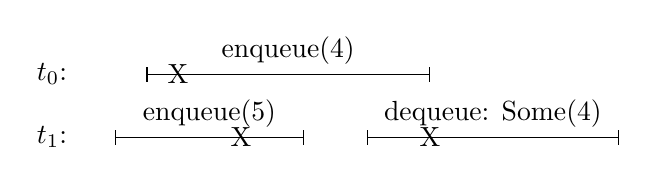
\begin{tikzpicture}[scale=0.8]
\draw (0,0) node {$t_0$:}; 
\draw[|-|] (1.5,0) -- node[above] {\scalashape enqueue(4)} (6,0);
\draw(2,0) node{X};
\draw (0,-1) node {$t_1$:}; 
\draw[|-|] (1,-1) -- node[above] {\scalashape enqueue(5)} (4,-1);
\draw(3,-1) node{X};
\draw[|-|] (5,-1) -- node[above] {\scalashape dequeue: Some(4)} (9,-1);
\draw(6,-1) node{X};
\end{tikzpicture}


Note that the history
\begin{scala}
  enqueue(4), enqueue(5), dequeue: Some(4)
\end{scala}
would be valid on a corresponding sequential queue. 
\end{slide}

%%%%%

\begin{slide}
\heading{Linearization examples}

But with different linearization points, a dequeue of 5 might have happened.

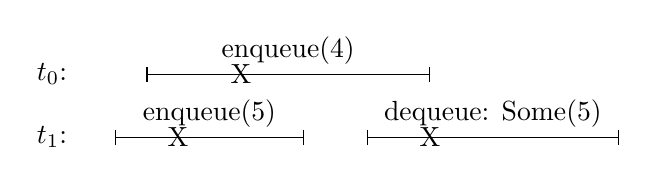
\begin{tikzpicture}[scale=0.8]
\draw (0,0) node {$t_0$:}; 
\draw[|-|] (1.5,0) -- node[above] {\scalashape enqueue(4)} (6,0);
\draw(3,0) node{X};
\draw (0,-1) node {$t_1$:}; 
\draw[|-|] (1,-1) -- node[above] {\scalashape enqueue(5)} (4,-1);
\draw(2,-1) node{X};
\draw[|-|] (5,-1) -- node[above] {\scalashape dequeue: Some(5)} (9,-1);
\draw(6,-1) node{X};
\end{tikzpicture}

Again note that the history
\begin{scala}
  enqueue(5), enqueue(4), dequeue: Some(5)
\end{scala}
would be valid on a corresponding sequential queue. 
\end{slide}

%%%%%

\begin{slide}
\heading{Linearization examples}

With the following timeline, the dequeue must return 5: any other return would
not be linearizable.
%
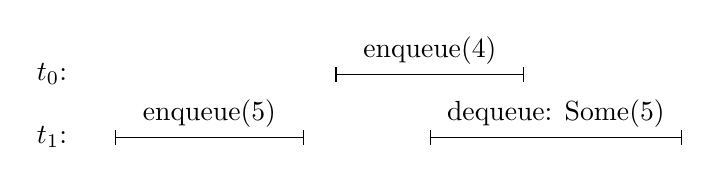
\begin{tikzpicture}[scale=0.8]
\draw (0,0) node {$t_0$:}; 
\draw[|-|] (4.5,0) -- node[above] {\scalashape enqueue(4)} (7.5,0);
%\draw(3,0) node{X};
\draw (0,-1) node {$t_1$:}; 
\draw[|-|] (1,-1) -- node[above] {\scalashape enqueue(5)} (4,-1);
%\draw(2,-1) node{X};
\draw[|-|] (6,-1) -- node[above] {\scalashape dequeue: Some(5)} (10,-1);
%\draw(6,-1) node{X};
\end{tikzpicture}

And the following history is not linearizable, because the queue is non-empty
throughout $t_2$'s operation.
%
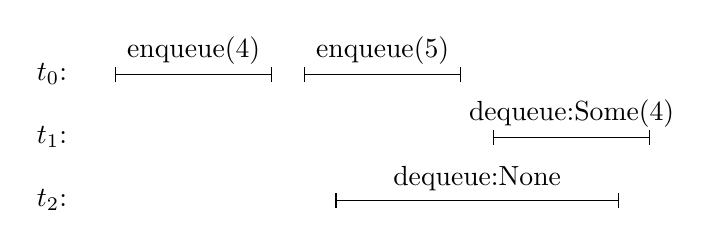
\begin{tikzpicture}[scale=0.8]
\draw (0,0) node {$t_0$:}; 
\draw[|-|] (1,0) -- node[above] {\scalashape enqueue(4)} (3.5,0);
\draw[|-|] (4,0) -- node[above] {\scalashape enqueue(5)} (6.5,0);
\draw (0,-1) node{$t_1$:};
\draw[|-|] (7,-1) -- node[above] {\scalashape dequeue:Some(4)} (9.5,-1);
\draw (0,-2) node{$t_2$:};
\draw[|-|] (4.5,-2) -- node[above] {\scalashape dequeue:None} (9,-2);
\end{tikzpicture}
\scalaMid
\end{slide}

%%%%%


%%%%%

\begin{slide}
\heading{Synchronous channels}

It is important that we use \emph{synchronous channels} in the server-based
queue.  Suppose we used buffered channels.  Then the following behaviour is
possible.
%
\begin{enumerate}
\item Thread $t_1$ calls |enqueue(5)|, but the value~|5| stays in the
  |enqueueChan|, even after $t_1$ returns;

\item Thread $t_2$ calls |dequeue|, and the server sends it |None|.
\end{enumerate}

Alternatively
%
\begin{enumerate}
\item The server sends |None| on |dequeueChan|, and that value stays in the
  channel; 

\item Thread $t_1$ calls |enqueue(5)|, and this value is received and stored
  by the server; 

\item Thread $t_2$ calls |dequeue|, and receives the |None| sent earlier.
\end{enumerate}
\end{slide}

%%%%%

\begin{slide}
\heading{Synchronous channels}

Using synchronous channels, the invocations have an effect in the order of the
channel communications.  This order is compatible with the order of the
invocations calls and returns.

We will always use synchronous channels when implementing a concurrent
datatype using a server process.   
\end{slide}


%%%%%

\begin{slide}
\heading{Testing for linearizability}

How can we test for linearizability?

Basic idea: 
%
\begin{itemize}
\item Run some threads on the concurrent queue, performing random |enqueue|
and |dequeue| operations, and record the history of operation calls and
returns;

\item Search for a corresponding sequential history that explains
linearizability, and that is a valid history for the corresponding sequential
datatype.  If none is found, signal an error.
\end{itemize}
%
Repeat many times.
\end{slide}

%%%%%

\begin{slide}
\heading{Testing for linearizability}

I've developed a framework to support such testing\footnote{{Testing
    for Linearizability}, Gavin Lowe, \textit{Concurrency and Computation},
    Practice and Experience, 29 (4), 2017,
  \url{http://www.cs.ox.ac.uk/people/gavin.lowe/LinearizabiltyTesting/}.},
and, in particular, investigated algorithms for testing whether a concurrent
history is linearizable.

In the next slides, we'll see a stripped-down testing script that uses this
(the full version can be used with multiple concurrent queue implementations,
and replaces the numerical constants by variables, specifiable via the command
line).

\vfill
\end{slide}

%%%%%

\begin{slide}
\heading{A small testing script}

The test program works on a concurrent datatype of some type~|C|; here we use
a |TotalQueue| containing |Int|s.  The test program
also requires a corresponding, \emph{immutable, deterministic}
sequential specification datatype~|S|, here an immutable queue from the Scala
API.
%
\begin{scala}
object QueueTest{
  type C = TotalQueue[Int]
  type S = scala.collection.immutable.Queue[Int]
  ...
}
\end{scala}
\end{slide}

%%%%%

\begin{slide}
\heading{A small testing script}

For each operation |op : A| on the concurrent datatype, we need a
corresponding function |seqOp : S => (A, S)| on the sequential datatype, which
returns the same value as the concurrent operation\footnote{More precisely,
  the two values should be equal, as tested using the ``{\scalashape ==}''
  method.}, paired with the new value of the sequential datatype.  These are
normally simple wrappers around API code.
%
\begin{scala}
  def seqEnqueue(x: Int)(q: S) : (Unit, S) = ((), q.enqueue(x))
  def seqDequeue(q: S) : (Option[Int], S) =   
    if(q.isEmpty) (None, q) 
    else{ val (r,q1) = q.dequeue; (Some(r), q1) }
\end{scala}
\vfill
\end{slide}

%%%%%

\begin{slide}
\heading{A small testing script}

The main part of the test program is the definition of a |worker| function
that performs and logs operations on the concurrent datatype, associating each
concurrent operation with a corresponding operation on the sequential
datatype.  Here, the worker performs 200 operations; each is (with probability
0.3) an enqueue of a random value, or (with probability~0.7) a dequeue.
\begin{scala}
  def worker(me: Int, log: LinearizabilityLog[S, C]) = {
    val random = new scala.util.Random
    for(i <- 0 until 200)
      if(random.nextFloat <= 0.3){
        val x = random.nextInt(20)
        log(_.enqueue(x), s"enqueue($x)", seqEnqueue(x))
      }
      else log(_.dequeue, "dequeue", seqDequeue)
  }
\end{scala}
\end{slide}

%%%%%

\begin{slide}
\heading{A small testing script}

The worker takes a log object |log| as a parameter; each operation is
performed and logged via a call to |log|, taking three parameters:
%
\begin{itemize}
% \item
% The identity of the thread doing the operation;

\item
The operation to be performed on the concurrent datatype;

\item A string describing the operation (this is used in debugging output in
the case that a non-linearizable history is found, and is also used internally
for optimisations; semantically different operations should have different
strings);

\item
The corresponding operation on the sequential datatype.
\end{itemize}

The call to |log| logs the invocation of the concurrent operation,
performs the concurrent operation, and logs the result returned.
\end{slide}
\begin{slide}
\heading{A small testing script}

The main test for linearizability is performed at line~\ref{line:maintest},
below, repeated so as to consider 1000 histories.  The  tester
takes as arguments: the sequential datatype; the concurrent datatype; the
number |p| of worker threads to run; and the definition of a worker thread.
%
\begin{scala}[numbers=left,numberstyle=\scriptsize]
  def main(args: Array[String]) = for(i <- 0 until 1000){
    val concQueue = new ServerTotalQueue[Int] // The concurrent queue
    val seqQueue = Queue[Int]() // The sequential specification queue
    val tester = LinearizabilityTester[S, C](seqQueue, concQueue, 4, worker _)
    assert(tester() > 0)£\label{line:maintest}£
  }
\end{scala}
%
The linearizability tester runs |p| workers concurrently, logging the
operation calls on the concurrent datatype.  It then tests whether the
resulting history is linearizable, returning a positive result if so.
\end{slide}

%%%%%

\begin{slide}
\heading{Controlling the search space}

The algorithm for testing linearizabilty, in effect, considers all possible
linearizations of the history, i.e.~all ways of ordering the operations
consistent with the history.  It then tests whether that ordering is
compatible with the sequential datatype, i.e.~whether performing the
corresponding sequential operations in the same order would give the same
results. 

Thus the algorithm considers all  states that the sequential
specification object could get into after a prefix of such linearizations.
%
If there are too many such states, this will take a long time.  It's therefore
a good idea to design the test so that such bad cases are very unlikely.
\end{slide}

%%%%%

\begin{slide}
\heading{Controlling the search space}

With a queue, the linearizability tester considers all possible states of the
sequential queue formed by permuting concurrent enqueue operations.  This
number grows exponentially with the length of the queue.  We therefore try to
avoid the length of the queue growing too much.  We did this in the earlier
testing harness by making dequeues more frequent than enqueues.
\end{slide}

%%%%%

\begin{slide}
\heading{Logging}

By default, the linearizability tester logs operation calls and returns using
thread-local logs, pairing each event with a timestamp.  We saw a similar
technique in an earlier chapter.  If you're using an operating system that
doesn't support timestamps property, setting the optional parameter |tsLog| to
|false| will use a different type of log.
%
\begin{scala}
  val tester = LinearizabilityTester[S, C](
    seqQueue, concQueue, 4, worker _, £\scalastyle\color{red} tsLog = false£)
\end{scala}
\end{slide}

%%%%%

%% \begin{slide}
%% \heading{Exercise}

%% Implement and test a total concurrent stack using similar techniques.
%% \end{slide}
 % concurrent total queue, using a server;
% linearizability testing



\begin{slide}
\heading{A partial queue}

In the previous chapter we implemented a total concurrent queue that returns
|None| if |dequeue| is called when the queue is empty.  
%
An alternative is to block that thread until there is a value to be dequeued.
This gives a partial queue, with the following interface.

\begin{scala}
trait PartialQueue[T]{
  /** Enqueue x. */
  def enqueue(x: T): Unit

  /** Dequeue a value.  Blocks until the queue is non-empty. */
  def dequeue: T

  /** Shut down the queue. */
  def shutdown
}
\end{scala}
Note that if the queue is empty and all threads are attempting a dequeue, the
system will deadlock. 
\end{slide}

%%%%%

\begin{slide}
\heading{A partial queue}

\begin{scala}
class ServerPartialQueue[T] extends PartialQueue[T]{
  // Channel for dequeueing
  private val dequeueChan = new SyncChan[T]

  def dequeue: T = dequeueChan?()

  private def server = thread{
    val queue = new scala.collection.mutable.Queue[T]
    serve(
      enqueueChan =?=> { x => queue.enqueue(x) }
      | queue.nonEmpty && dequeueChan =!=> queue.dequeue
    )
  }

  ... // other parts as earlier
}
\end{scala}
\end{slide}

%%%%%

\begin{slide}
\heading{Testing}

We can test this queue for linearizability, much as for the previous version.
However, we have to amend the sequential specification object to recognise
that a dequeue cannot happen when the queue is empty. 
\begin{scala}
  def seqDequeue(q: S) : (Int, S) = {
    require(q.nonEmpty); q.dequeue
  }
\end{scala}
An operation invocation on the concurrent datatype cannot be linearized in a
state where the corresponding operation on the sequential datatype throws an
|IllegalArgumentException|.

Also we have to be careful that we never get into a deadlocked state where all
the threads are attempting a dequeue from the empty queue.  I arrange for half
the threads to perform just enqueues, and the others to perform just dequeues.  
\end{slide}

%%%%%

\begin{slide}
\heading{Termination}

Suppose the queue is empty, and all the threads are attempting a dequeue.
With the previous design, the system would be deadlocked.

A better approach would be for the server to detect such a state, and react
accordingly.  We choose to shut down the queue in this case, and arrange for
each dequeue attempt to throw a |Stopped| exception (an alternative would be
to use an |Option| value).

In order to do this, the server needs to know how many threads are attempting
a dequeue.  That means we can't just block the |dequeueChan| channel when the
queue is empty.  Instead, we arrange for the dequeueing thread to pass a reply
channel on the |dequeueChan|.  These reply channels are stored until the
request can be made.  If the number of stored reply channels equals the number
of workers, the queue shuts down.
\end{slide}

%%%%%

\begin{slide}
\heading{Termination}

\begin{scala}
/** A partial queue that terminates if all worker threads are attempting to
  * dequeue, and the queue is empty.
  * @param numWorkers the number of worker threads. */
class TerminatingPartialQueue[A](numWorkers: Int){
  private type ReplyChan = Chan[A]
  /** Channel for dequeueing. */
  private val dequeueChan = new SyncChan[ReplyChan]

  /** Attempt to dequeue a value.
    * @throws Stopped exception if the queue has been shutdown. */
  def dequeue: A = {
    val reply = new SyncChan[A] // or a BuffChan[A]
    dequeueChan!reply
    reply?()
  }
  ... 
}
\end{scala}
\end{slide}

%%%%%

\begin{slide}
\heading{Termination}

We might also want to externally shut down the server, (e.g.~in a search
algorithm, if we find what we're looking for).

It's necessary for the server to control termination in this case, so we
arrange for the |shutdown| method to send a message to the server. 
%
\begin{scala}
  private val shutdownChan = new SyncChan[Unit]

  /** Shut down this queue. */
  def shutdown = attempt{ shutdownChan!(()) }{ }
\end{scala}
Note: it's possible that the server has already terminated and |shutdownChan|
closed, in which case we catch the |Stopped| exception.

%% The construct
%% \begin{scala}
%%   attempt{ p }{ q }
%% \end{scala}
%% Executes |p|; but if |p| throws a |Stopped| exception, that exception is
%% caught, and |q| is executed. 
\end{slide}
  
%%%%%

\begin{slide}
\heading{The server}

\begin{scala}
  private def server = thread("server"){
    // Currently held values
    val queue = new Queue[A]()
    // Queue holding reply channels for current dequeue attempts.
    val waiters = new Queue[ReplyChan]()
    // Invariant: queue.isEmpty or waiters.isEmpty

    // Termination: signal to all waiting workers
    def close = {
      for(c <- waiters) c.close
      enqueueChan.close; dequeueChan.close; shutdownChan.close
    }
    ...
  }
\end{scala}
\end{slide}

%%%%%

\begin{slide}
\heading{The server main loop}

\begin{scala}
    serve(
      enqueueChan =?=> { x => 
        if(waiters.nonEmpty){ // pass x directly to a waiting dequeue
          assert(queue.isEmpty); waiters.dequeue!x
        }
        else queue.enqueue(x)
      }
      | dequeueChan =?=> { reply =>
          if(queue.nonEmpty) reply!(queue.dequeue) // service request immediately
          else{                                        // thread has to wait
            waiters.enqueue(reply)
            if(waiters.length == numWorkers) close
          }
        }
      | shutdownChan =?=> { _ => close }
    )
\end{scala}
\end{slide}
 % partial queue, including termination

\begin{slide}
\heading{Example: graph search}

Many Computer Science applications involve searching in a graph (whether
explicitly or implicitly).  Examples:
%
\begin{itemize}
\item Route planning;

\item Planning;

\item Puzzle solving;

\item Verification.
\end{itemize}
%
Searches might aim to minimise some cost, or might aim to find a node with a
particular property, using breadth-first search or depth-first search.

We will examine an algorithm for (approximate) concurrent breadth-first search.

The third practical asks you to implement (approximate) concurrent depth-first search.
\end{slide}

%%%%%

\begin{slide}
\heading{Graphs and graph search}

For our purposes, a graph can be defined by a function that gives all the
successors (or neighbours) of a given node.
%
\begin{scala}
/** A trait representing an unlabelled graph with nodes of type N. */
trait Graph[N]{
  /** The successors of node n.  All nodes n' such that there is an edge
    * from n to n' */
  def succs(n: N): List[N]
}
\end{scala}

We will search from some start node to try to find a path to a node with a
particular property |isTarget|.
\begin{scala}
/** Trait representing a graph search problem in graph g. */
abstract class GraphSearch[N](g: Graph[N]){
  /** Try to find a path in g from start to a node that satisfies isTarget. */
  def apply(start: N, isTarget: N => Boolean): Option[List[N]]
}
\end{scala}
\end{slide}

%%%%%

\begin{slide}
\heading{Example}

\def\word#1{\emph{#1}}
A popular word game, invented by Lewis Carroll, is to find a path of words,
each differing from the previous in a single letter, linking two given words.
Carroll used the example of finding such a path linking \word{grass} to
\word{green}, and gave the solution \word{grass}, \word{crass}, \word{cress},
\word{tress}, \word{trees}, \word{frees}, \word{freed}, \word{greed},
\word{green}, although in fact there are shorter solutions.

The course website contains a solution to this problem.  A |Graph| is built,
with words (from some dictionary file) as nodes, and with the successors of a
node being those that differ by one letter.  The |GraphSearch| then solves the
problem.
\end{slide}

%%%%%

\begin{slide}
\heading{Sequential breadth-first graph search}

We will search the graph in breadth-first order.  We will use a queue to store
nodes that still need to be expanded: this provides the breadth-first
behaviour.  Each node will be paired with the path that reached it, to allow a
successful path to be reproduced.

In addition, we will keep track of the set of nodes seen previously, to avoid
repeating work.
\begin{scala}
/** Sequential graph search implementation. */
class SeqGraphSearch[N](g: Graph[N]) extends GraphSearch[N](g){
  def apply(start: N, isTarget: N => Boolean): Option[List[N]] = {
    // Queue storing nodes and the path leading to that node
    val queue = new scala.collection.mutable.Queue[(N, List[N])]()
    queue += ((start, List(start)))
    // All nodes seen so far.
    val seen = scala.collection.mutable.Set[N](start)
    ...
} }
\end{scala}
\end{slide}

%%%%%

\begin{slide}
\heading{Sequential breadth-first graph search}

We repeatedly remove a node from the queue, and consider each of its
successors.  If a successor node is a target, we are done.  Otherwise, if the
successor node hasn't been seen previously, we add it to the queue.
%
\begin{scala}
  def apply(start: N, isTarget: N => Boolean): Option[List[N]] = {
    ...
    while(queue.nonEmpty){
      val (n, path) = queue.dequeue
      for(n1 <- g.succs(n)){
        if(isTarget(n1)) return Some(path :+ n1)
        else if(seen.add(n1)) queue.enqueue((n1, path :+ n1))
      }
    }
    None
  }
\end{scala}
\end{slide}

%%%%%

\begin{slide}
\heading{Towards a concurrent algorithm}

We will implement a concurrent algorithm where each worker thread will execute
very much as in the main loop of the sequential algorithm.

The workers will share a concurrent queue.  We will use a
|TerminatingPartialQueue|. 

The workers will also share a concurrent set, with the following interface.
Exercise: implement such a set.
%
\begin{scala}
class ConcSet[A]{
  /** Add x to this set.  Return true if x was not previously in the set. */
  def add(x: A): Boolean
}
\end{scala}

We also assume that the |succs| method on the |Graph| object is thread-safe.
In most cases, this method will just perform reads, so there will be no race
conditions. 
\end{slide}

%%%%%

\begin{slide}
\heading{Towards a concurrent algorithm}

\begin{scala}
/** A class to search Graph g concurrently. */
class ConcGraphSearch[N](g: Graph[N]) extends GraphSearch[N](g){
  /**The number of workers. */
  val numWorkers = 8

  /** Try to find a path in g from start to a node that satisfies isTarget. */
  def apply(start: N, isTarget: N => Boolean): Option[List[N]] = {
    // Queue storing nodes and the path leading to that node
    val queue = new TerminatingPartialQueue[(N, List[N])](numWorkers)
    queue.enqueue((start, List(start)))
    // All nodes seen so far.
    val seen = new ConcSet[N]; seen.add(start)
    ...
  }
}
\end{scala}
\end{slide}

%%%%%

\begin{slide}
\heading{Termination}

There are a few complications concerning termination.
%
\begin{itemize}
\item If a path is found, we need to arrange for that path to be returned.  If
two threads each find a path, we need to return just one of them.  We need to
ensure the other threads terminate, and the queue is shut down.

We will use a |coordinator| thread to help with this.  If a thread finds a
path, it will send it to the |coordinator|.

\item If no path exists, we will get to a state where the queue is empty and
all threads are trying to dequeue a node; the |TerminatingPartialQueue| will
help us to terminate.
\end{itemize}
\end{slide}

%%%%%

\begin{slide}
\heading{A worker}

\begin{scala}
    // Channel on which a worker tells the coordinator that it has found a
    // solution.
    val pathFound = ManyOne[List[N]]

    // A single worker
    def worker = thread("worker"){
      repeat{
        val (n, path) = queue.dequeue
        for(n1 <- g.succs(n)){
          if(isTarget(n1)) pathFound!(path :+ n1) // done!
          else if(seen.add(n1)) queue.enqueue((n1, path :+ n1))
        }
      }
      pathFound.close // causes coordinator to close down
    }
\end{scala}
\end{slide}

%%%%%

{\advance\slideheight by 3mm
\begin{slide}
\heading{The coordinator}

\begin{scala}
    // Variable that ends up holding the result; written by coordinator. 
    var result: Option[List[N]] = None

    def coordinator = thread("coordinator"){
      attempt{ result = Some(pathFound?()) }{ }
      queue.shutdown // close queue; this will cause most workers to terminate
      pathFound.close // in case another worker has found solution
    }
\end{scala}

If a thread finds a path, it sends it to the coordinator.  The coordinator
shuts down the queue and closes |pathFound|.  Any operation on the queue will
throw a |Stopped| exception.  Hence all the workers will terminate.  (It might
also be necessary to shut down the |seen| set.)

Alternatively, if there is no solution, the |queue| will eventually close
itself, throwing |Stopped| exceptions to the workers.  A worker will close
|pathFound|, so the coordinator will also terminate. 
\end{slide}}

%%%%%

\begin{slide}
\heading{Putting it together}

\begin{scala}
  def apply(start: N, isTarget: N => Boolean): Option[List[N]] = {
    ... // initialise queue and seen set.
    val workers = || (for(_ <- 0 until numWorkers) yield worker)
    run(workers || coordinator)
    result
  }
\end{scala}
\end{slide}

%%%%%

\begin{slide}
\heading{Breadth-first search}

This doesn't quite achieve breadth-first search.  If a thread is delayed,
deeper nodes might be explored while a node from an earlier ply is being
expanded.  This might mean that the path that is found isn't the shortest.  In
many cases, this won't matter much.  If true breadth-first behaviour is
needed, the threads can performs a global synchronisation at the end of each
ply.
\end{slide}

%%%%%

\begin{slide}
\heading{Bag-of-tasks with replacement}

The implementation can be seen as a variant of the bag-of-tasks pattern, but
where additional tasks may be added to the bag.

Each node in the bag (the queue) represents the task of expanding that node.
This may lead to additional tasks being added to the bag.
\end{slide}
 % breadth-first search.

%%%%%

\begin{slide}
\heading{Summary}

\begin{itemize}
\item 
Concurrent datatypes;

\item
Total and partial datatypes;

\item
Linearization; testing for linearizability;

\item
Examples;

\item 
Termination;

\item Example: breadth-first search.
\end{itemize}
\end{slide}


\end{document}
